\let\negmedspace\undefined
\let\negthickspace\undefined
\documentclass[journal]{IEEEtran}
\usepackage[a5paper, margin=10mm, onecolumn]{geometry}
%\usepackage{lmodern} % Ensure lmodern is loaded for pdflatex
\usepackage{tfrupee} % Include tfrupee package

\setlength{\headheight}{1cm} % Set the height of the header box
\setlength{\headsep}{0mm}     % Set the distance between the header box and the top of the text

\usepackage{gvv-book}
\usepackage{gvv}
\usepackage{cite}
\usepackage{amsmath,amssymb,amsfonts,amsthm}
\usepackage{algorithmic}
\usepackage{graphicx}
\usepackage{textcomp}
\usepackage{xcolor}
\usepackage{txfonts}
\usepackage{listings}
\usepackage{enumitem}
\usepackage{mathtools}
\usepackage{gensymb}
\usepackage{comment}
\usepackage[breaklinks=true]{hyperref}
\usepackage{tkz-euclide} 
\usepackage{listings}
% \usepackage{gvv}                                        
\def\inputGnumericTable{}                                 
\usepackage[latin1]{inputenc}                                
\usepackage{color}                                            
\usepackage{array}                                            
\usepackage{longtable}                                       
\usepackage{calc}                                             
\usepackage{multirow}                                         
\usepackage{hhline}                                           
\usepackage{ifthen}                                           
\usepackage{lscape}
\begin{document}
\bibliographystyle{IEEEtran}
\vspace{3cm}

\title{5.5.12}
\author{EE25BTECH11060 - V.Namaswi}
% \maketitle
% \newpage
% \bigskip
{\let\newpage\relax\maketitle}
\renewcommand{\thefigure}{\theenumi}
\renewcommand{\thetable}{\theenumi}
\setlength{\intextsep}{10pt} % Space between text and floats
\textbf{Question}\\If $\Vec{A}=\begin{pmatrix}
 1 & 1 &  1\\
    1 & 0 &  2\\
    3  & 1 & 1 
\end{pmatrix}
$\\find $\Vec{A}^{-1}$ . Hence solve the following system of equations \\
\begin{align*}
   x+y+z=6\\
    x+2z=7\\
    3x+y+z=12 
\end{align*}
\textbf{Solution}\\
\begin{align}
\Vec{A} \Vec{x}=\vec{I}
\end{align}
Forming Argumented Matrix
\begin{align}
    \augvec{3}{3}{1 & 1 & 1 & 1 & 0 & 0\\
1 & 0 & 2 & 0 & 1 & 0\\
3 & 1 & 1 & 0 & 0 & 1}
\end{align}
Replace $R2 \to R2-R1$ and $R3 \to R3-3R1 $ \\
\begin{align}
\augvec{3}{3}{1 & 1 & 1 & 1 & 0 & 0\\
0 & -1 & 1 & -1 & 1 & 0\\
0 & -2 & -2 & -3 & 0 & 1} 
\end{align}
Replace $R2 \to -R2$ and $R3 \to R3+2R2 $\\
\begin{align}
    \augvec{3}{3}{ 1 & 0 & 2 & 0 & 1 & 0\\
0 & 1 & -1 & 1 & -1 & 0\\
0 & 0 & -4 & -1 & -2 & 1
}
\end{align}
Repalce  \(R_3\leftarrow -\tfrac{1}{4}R_3\)
\begin{align}
    \augvec{3}{3}{1 & 0 & 2 & 0 & 1 & 0\\
0 & 1 & -1 & 1 & -1 & 0\\
0 & 0 & 1 & \tfrac14 & \tfrac12 & -\tfrac14}
\end{align}
Replace \(R_1\leftarrow R_1-2R_3,\; R_2\leftarrow R_2+R_3\)
\begin{align}
    \augvec{3}{3}{1 & 0 & 0 & -\tfrac12 & 0 & \tfrac12\\
0 & 1 & 0 & \tfrac54 & -\tfrac12 & -\tfrac14\\
0 & 0 & 1 & \tfrac14 & \tfrac12 & -\tfrac14}
\end{align}
Thus
\begin{align}
A^{-1}=\begin{pmatrix}
-\tfrac12 & 0 & \tfrac12\\[6pt]
\tfrac54 & -\tfrac12 & -\tfrac14\\[6pt]
\tfrac14 & \tfrac12 & -\tfrac14
\end{pmatrix}.
\end{align}
\begin{align}
   \vec{X}=\vec{A^{-1}} \vec{b}\\
   \vec{X}
   =\begin{pmatrix}
-\tfrac12 & 0 & \tfrac12\\[4pt]
\tfrac54 & -\tfrac12 & -\tfrac14\\[4pt]
\tfrac14 & \tfrac12 & -\tfrac14
\end{pmatrix}
\begin{pmatrix}6\\[2pt]7\\[2pt]12\end{pmatrix}\\
\vec{X}=\begin{pmatrix}
    3 \\ 1 \\ 2
\end{pmatrix}
\end{align}
    \centering
    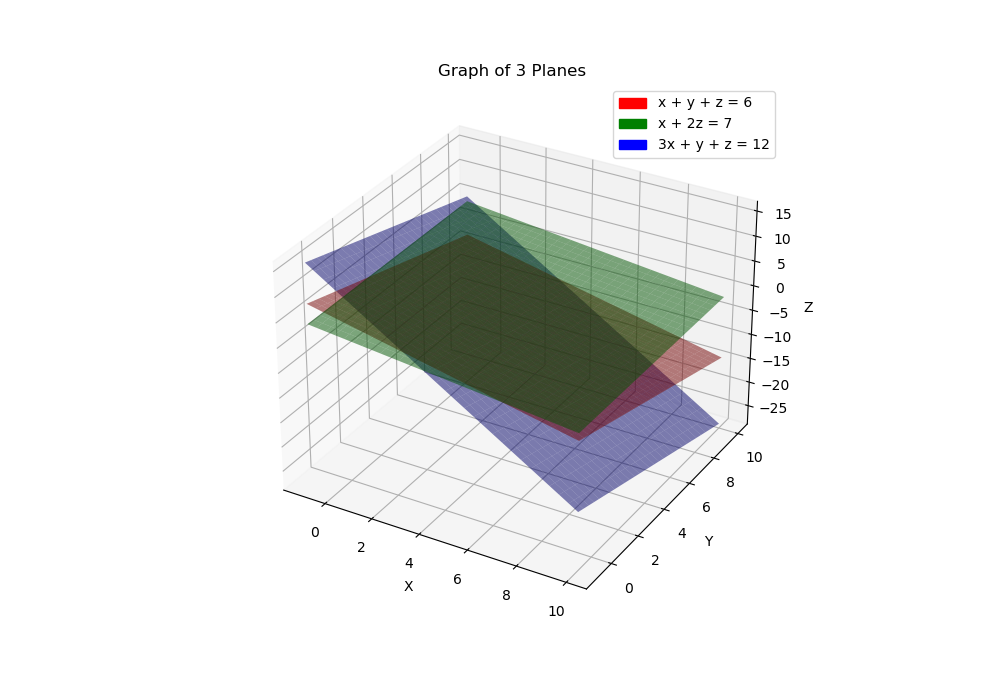
\includegraphics[width=\columnwidth, height=0.8\textheight, keepaspectratio]{figs/Figure_11.png}    
\end{document}